\documentclass[12pt]{article}
\usepackage[utf8]{inputenc}
\usepackage{float}
\usepackage{amsmath}


\usepackage[hmargin=3cm,vmargin=6.0cm]{geometry}
%\topmargin=0cm
\topmargin=-2cm
\addtolength{\textheight}{6.5cm}
\addtolength{\textwidth}{2.0cm}
%\setlength{\leftmargin}{-5cm}
\setlength{\oddsidemargin}{0.0cm}
\setlength{\evensidemargin}{0.0cm}

%misc libraries goes here
\usepackage{tkz-euclide}


\begin{document}

\section*{Student Information } 
%Write your full name and id number between the colon and newline
%Put one empty space character after colon and before newline
Full Name :  Abdulkadir Pamukçu \\
Id Number :  2237774 

% Write your answers below the section tags
\section*{Answer 1}
\subsection*{a)}
Since every 1 is followed immediately 1 is followed by a 0, let us take "10" as an one element. After that we need to examine all possible situations and sum all of them and find the answer.\\
\\
1-) If string contains only one "10":\\
String of length 8 and contains one "10" and seven "0" For to choose location of "10"  :\\
${8 \choose 1}$ = 8 \\ 
2-) If string contains two "10":\\
String of length 7 and contains two "10" and five "0" For to choose location of "10" s :\\
${7 \choose 2}$ = 21 \\ 
3-) If string contains three "10":\\
String of length 6 and contains three "10" and three "0" For to choose location of "10" s :\\
${6 \choose 3}$ = 20 \\ 
4-) If string contains four "10":\\
String of length 5 and contains four "10" and one "0" For to choose location of "10" s :\\
${5 \choose 4}$ = 5 \\ 
\\ Hence: There are 8+20+21+5= 54 possible strings.
\subsection*{b)}
In this question there are 3 possible cases: ten of ten, nine of ten and eight of ten are 1s.\\
\\For 10 of 10 are 1s. To choose them:\\
This means all of them is 1:\\
${10 \choose 10}$ = 1\\
\\For 10 of 9 are 1:\\
This means one of them is 0 and 9 of them is 1s. To choose them :\\
${10 \choose 9}$ = 10 also the 0's are identical so it doesn't make any difference so = 10.\\ 
\\For 10 of 8 are 1:\\
This means two of them is 0s and eight of them is 1s. To choose them :\\
${10 \choose 8}$ = 45 also the 0's are identical so it doesn't make any difference so = 45.\\ 
\\
Hence: There 1+45+10=56 bit strings of length 10 have at least eight of them 1s.
\subsection*{c)}
Since onto functions means there is no empty element in image set. Also considering the function restrictions. One of the elements in image set need to be image of two elements in domain set. There is 3 cases. To find the answer we need to calculate them all:\\
1-) First element in image set is image of 2 elements in domain set. And others images of other elements in domain set. To choose them:\\
${4 \choose 2}$ * ${2 \choose 1}$ * ${1 \choose 1}$ = 12\\
2-) Second element in image set is image of 2 elements in domain set. And others images of other elements in domain set. To choose them:\\
${4 \choose 1}$ * ${3 \choose 2}$ * ${1 \choose 1}$ = 12\\
3-) Third element in image set is image of 2 elements in domain set. And others images of other elements in domain set. To choose them:\\
${4 \choose 1}$ * ${3 \choose 1}$ * ${2 \choose 2}$ = 12\\
\\
Therefore, there are 12+12+12 = 36 onto functions.\\
\subsection*{d)}
Since in collection there must be at least one Discrete Mathematics textbook and at least one Signals and Systems textbook according to the question. So all we need to figure out is how many ways to choose remaining two books. It can be done in 3 ways:\\
1- Discrete Mathematics textbook and Signals and Systems textbook\\
2- Two Signals and Systems textbooks\\
3- Two Discrete Mathematics textbooks\\
\\Therefore there are 3 ways.


\section*{Answer 2}
\subsection*{a)}
Let's split up $a_n$. $a_n$  = number of subsets of the set {1,2,3..,n} that don't contain two consecutive numbers and also contains n +  number of subsets of the set {1,2,3..,n} that don't contain two consecutive number but do not contain n.\\
The number of subsets of the set {1,2,3..,n} that don't contain two consecutive number do not contain n equals to the number of subsets of the set {1,2,3...,n-1} that don't contain two consecutive number. And that is also equal to $a_{n-1}$  \\
The number of subsets of the set {1,2,3..,n} that don't contain two consecutive numbers and also contains n equals to the number of subsets of the set {1,2,3..n} that do not contain two consecutive numbers and also not including n-1 since there can't be two consecutive numbers if it is contains n it can't include n-1\\
And the number of subsets of the set {1,2,3..n} that do not contain two consecutive numbers and also not including n-1  equals to the number of subsets of the set {1,2,3...,n-2} that don't contain two consecutive numbers. and that is also equal to $a_{n-2}$ \\
Therefore:\\
For all n$>$2  $a_{n}$ = $a_{n-1}$ +$a_{n-2}$
\subsection*{b)}





\section*{Answer 3}

The characteristic equation of this recurrence relation is: $r^3$ - 4$r^2$ - $r$  + 4 = 0\\
4,1,-1 are the roots of this characteristic equation. Hence, the sequence a$_n$
is a solution to the recurrence relation if and only if:\\
a$_n$ = c$_1$4$^n$ + c$_2$1$^n$ +  c$_3$(-1)$^n$\\
Since we know $a_0$ = 4, $a_0$ = 4 = c$_1$4$^0$ + c$_2$1$^0$ +  c$_3$(-1)$^0$ \\ c$_1$+c$_2$+c$_3$ = 4\\
Also $a_1$ = 4, $a_1$ = 8 = c$_1$4$^1$ + c$_2$1$^1$ +  c$_3$(-1)$^1$\\ 4c$_1$+c$_2$-c$_3$ = 8\\
Also $a_2$ = 34, $a_2$ = 34 = c$_1$4$^2$ + c$_2$1$^2$ +  c$_3$(-1)$^2$\\ 16c$_1$+c$_2$+c$_3$ = 34\\
We now find c$_1$=2, c$_2$ = 1, c$_3$ = 1\\
Therefore we find recurrence relation is: a$_n$ = 2x4$^n$ + 1$^n$ +  (-1)$^n$\\

\section*{Answer 4}
\subsection*{a)}
There is three condition for a relation to be equivalence relation. It need to be reflexive, symmetric and transitive. To prove we need to check all three.\\
\\
1- Reflexive: For (a$_1$,b$_1$) ; 3a$_1$ - 2b$_1$ = 3a$_1$ - 2b$_1$ is true. Therefore this relation R is reflexive.\\
2- Symmetric: 3x$_1$ - 2y$_1$ = 3x$_2$ - 2y$_2$ implies 3x$_2$ - 2y$_2$ = 3x$_1$ - 2y$_1$ is holds true. Thus this relation R is symmetric. \\
3- Transitive: (3x$_1$ - 2y$_1$ = 3x$_2$ - 2y$_2$ and 3x$_2$ - 2y$_2$ = 3x$_3$ - 2y$_3$) implies 3x$_1$ - 2y$_1$ = 3x$_3$ - 2y$_3$ is also true. Hence this relation R is also transitive.\\
\\
Since R reflexive, symmetric and transitive. by showing these we prove R is an equivalence relation.
\subsection*{b)}



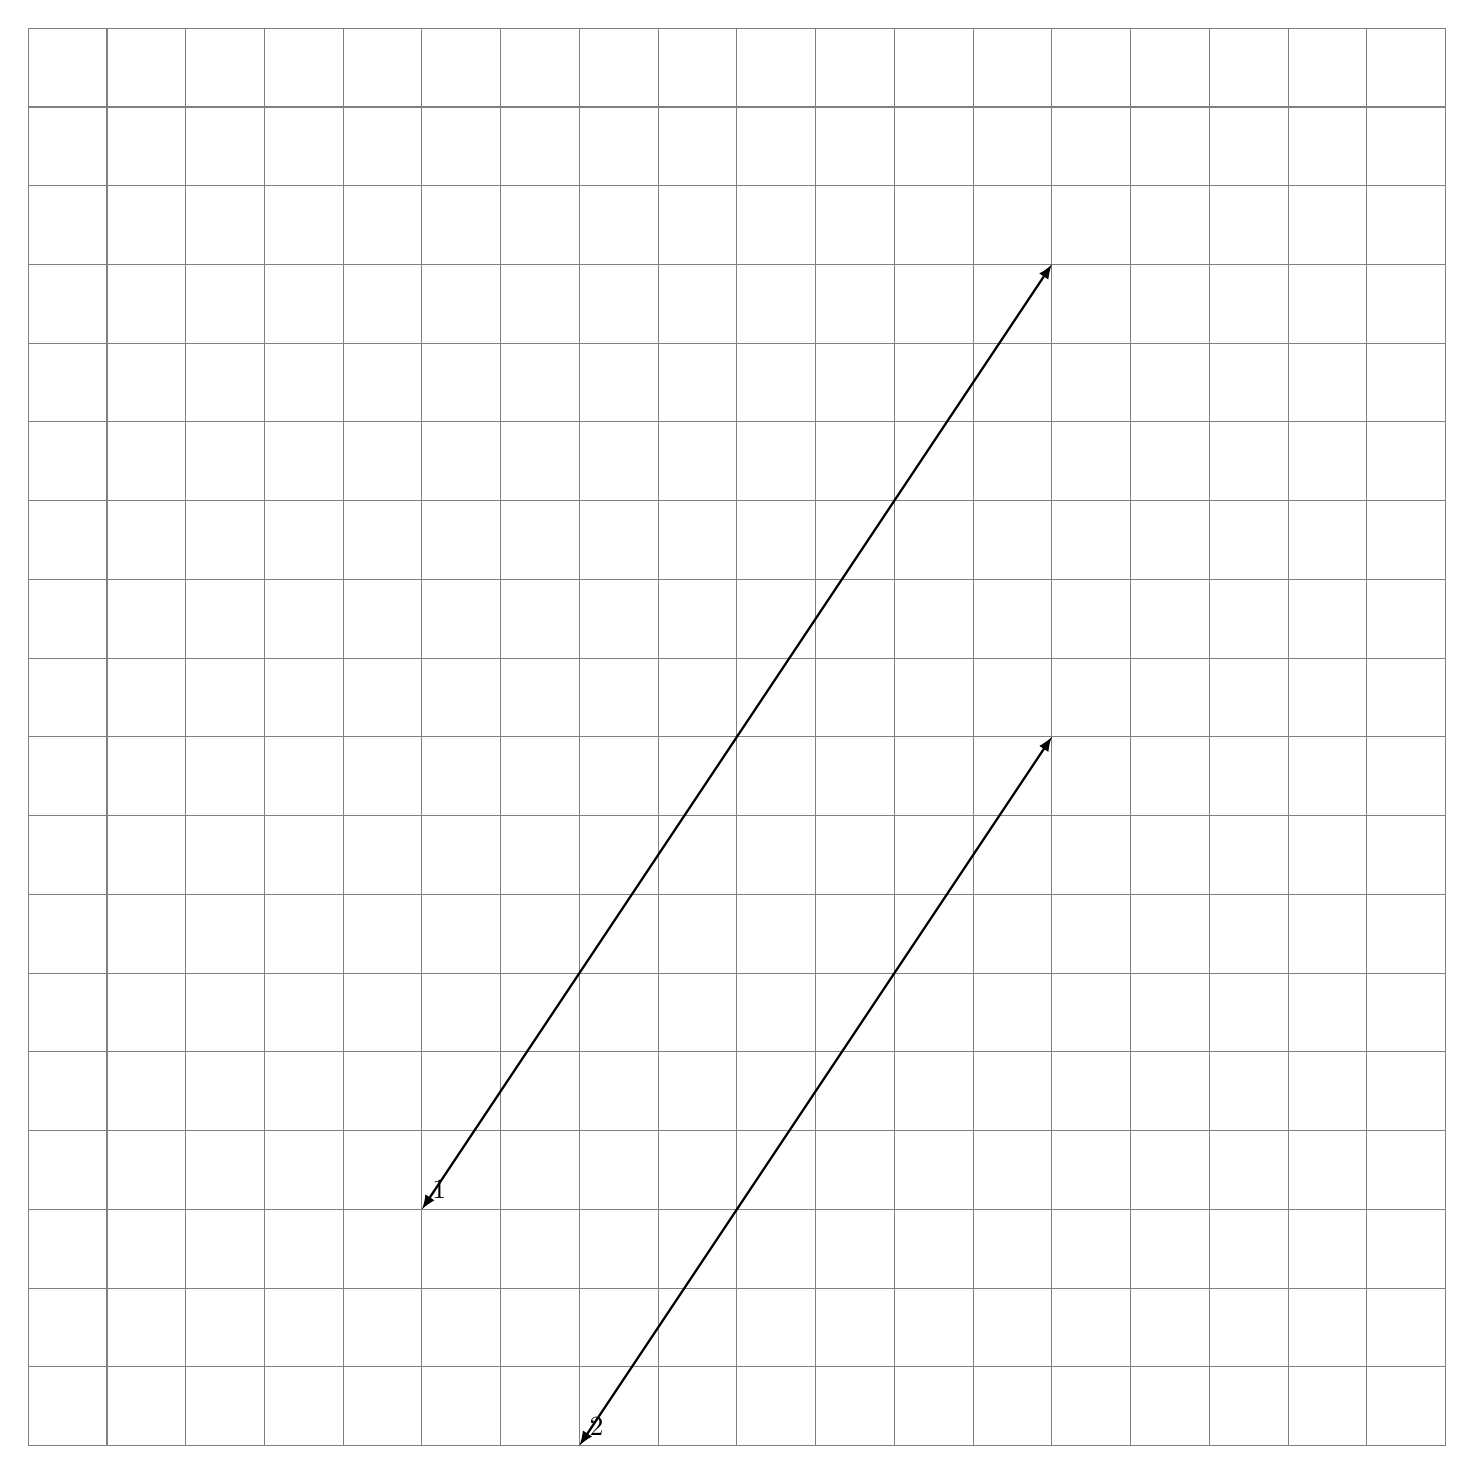
\begin{tikzpicture}
   \tkzInit[xmax=9,ymax=9,xmin=-9,ymin=-9]
   \tkzGrid
   \tkzAxeXY
   \draw[ thick,latex-latex] (4,6) -- (-4,-6) node[anchor=south west] {$1$}; % two points for
   \draw[ thick,latex-latex] (4,0) -- (-2,-9) node[anchor=south west] {$2$};
   drawing 2x+y=2
  \tkzText[above](0,6.75){}
  \end{tikzpicture}


\end{document}